\documentclass[a4paper, 11pt]{article}
\usepackage[UTF8]{ctex}
%%%%%% 导入包 %%%%%%
\usepackage{CJKutf8}

\usepackage{graphicx}
\usepackage[unicode]{hyperref}
\usepackage{xcolor}
\usepackage{cite}
\usepackage{indentfirst}
%\usepackage{ctex}
%%%%%% 设置字号 %%%%%%
\newcommand{\chuhao}{\fontsize{42pt}{\baselineskip}\selectfont}
\newcommand{\xiaochuhao}{\fontsize{36pt}{\baselineskip}\selectfont}
\newcommand{\yihao}{\fontsize{28pt}{\baselineskip}\selectfont}
\newcommand{\erhao}{\fontsize{21pt}{\baselineskip}\selectfont}
\newcommand{\xiaoerhao}{\fontsize{18pt}{\baselineskip}\selectfont}
\newcommand{\sanhao}{\fontsize{15.75pt}{\baselineskip}\selectfont}
\newcommand{\sihao}{\fontsize{14pt}{\baselineskip}\selectfont}
\newcommand{\xiaosihao}{\fontsize{12pt}{\baselineskip}\selectfont}
\newcommand{\wuhao}{\fontsize{10.5pt}{\baselineskip}\selectfont}
\newcommand{\xiaowuhao}{\fontsize{9pt}{\baselineskip}\selectfont}
\newcommand{\liuhao}{\fontsize{7.875pt}{\baselineskip}\selectfont}
\newcommand{\qihao}{\fontsize{5.25pt}{\baselineskip}\selectfont}

%%%% 设置 section 属性 %%%%
\makeatletter
\renewcommand\section{\@startsection{section}{1}{\z@}%
	{-1.5ex \@plus -.5ex \@minus -.2ex}%
	{.5ex \@plus .1ex}%
	{\normalfont\sihao\CJKfamily{hei}}}
\makeatother

%%%% 设置 subsection 属性 %%%%
\makeatletter
\renewcommand\subsection{\@startsection{subsection}{1}{\z@}%
	{-1.25ex \@plus -.5ex \@minus -.2ex}%
	{.4ex \@plus .1ex}%
	{\normalfont\xiaosihao\CJKfamily{hei}}}
\makeatother

%%%% 设置 subsubsection 属性 %%%%
\makeatletter
\renewcommand\subsubsection{\@startsection{subsubsection}{1}{\z@}%
	{-1ex \@plus -.5ex \@minus -.2ex}%
	{.3ex \@plus .1ex}%
	{\normalfont\xiaosihao\CJKfamily{hei}}}
\makeatother

%%%% 段落首行缩进两个字 %%%%
\makeatletter
\let\@afterindentfalse\@afterindenttrue
\@afterindenttrue
\makeatother
\setlength{\parindent}{2em}  %中文缩进两个汉字位


%%%% 下面的命令重定义页面边距,使其符合中文刊物习惯 %%%%
\addtolength{\topmargin}{-54pt}
\setlength{\oddsidemargin}{0.63cm}  % 3.17cm - 1 inch
\setlength{\evensidemargin}{\oddsidemargin}
\setlength{\textwidth}{14.66cm}
\setlength{\textheight}{24.00cm}    % 24.62

%%%% 下面的命令设置行间距与段落间距 %%%%
\linespread{1.4}
% \setlength{\parskip}{1ex}
\setlength{\parskip}{0.5\baselineskip}

%%%% 正文开始 %%%%
\begin{document}
	
		
		%%%% 定理类环境的定义 %%%%
		\newtheorem{example}{例}             % 整体编号
		\newtheorem{algorithm}{算法}
		\newtheorem{theorem}{定理}[section]  % 按 section 编号
		\newtheorem{definition}{定义}
		\newtheorem{axiom}{公理}
		\newtheorem{property}{性质}
		\newtheorem{proposition}{命题}
		\newtheorem{lemma}{引理}
		\newtheorem{corollary}{推论}
		\newtheorem{remark}{注解}
		\newtheorem{condition}{条件}
		\newtheorem{conclusion}{结论}
		\newtheorem{assumption}{假设}
		
		%%%% 重定义 %%%%
		\renewcommand{\contentsname}{目录}  % 将Contents改为目录
		\renewcommand{\abstractname}{摘要}  % 将Abstract改为摘要
		\renewcommand{\refname}{参考文献}   % 将References改为参考文献
		\renewcommand{\indexname}{索引}
		\renewcommand{\figurename}{图}
		\renewcommand{\tablename}{表}
		\renewcommand{\appendixname}{附录}
		\renewcommand{\algorithm}{算法}
		
		
		%%%% 定义标题格式,包括title,author,affiliation,email等 %%%%
		\title{轻量化网络发展现状及其在遥感图像处理领域\\研究成果综述}
	%	\author{徐浩\footnote{电子邮件: xu_hao_98@163.com}\\[2ex]
		%	\xiaosihao 中国科学院计算技术研究所\\[2ex]
	%	}
		\author{徐浩\footnote{电子邮件: xu\_hao\_98@163.com}}
		\date{2020年10月}
		
		
		%%%% 以下部分是正文 %%%%  
		\maketitle
		\tableofcontents
		\newpage

\section{引言}
本次报告从研究目的,轻量化网络的国内外研究现状以及在遥感图像领域的应用现状,同时详细介绍当前采取的轻量化网络的主要策略。
\subsection{研究目的}
卷积神经网络在图像的分类、分割以及检测等领域都获得了广泛的应用,并且有着十分优异的检测性能,但随之而来的就是越来越深,越来越复杂的网络,这些网络模型虽然可以获得很好的检测效果,但过于复杂的模型以及过于多的参数和计算量,使得模型的部署成为了一个很大的问题,就是说一个好的深度学习模型无法部署在性能一般的硬件上,从AlexNet\cite{AlexNet}提出到现在已经八年了,中间出现了VGGNet\cite{VGGNet},ResNet\cite{ResNet},DenseNet\cite{DenseNet}等性能优异的网络结构,总的发展趋势就是网络的层数越来越深,一般情况下,网络越深,特征提取的能力越强,但是随之而来的是,中间会造成大量的特征冗余以及参数冗余,这就大大限制了网络的工业应用范围,因此,对神经网络进行轻量化是当前需要解决的问题,故对轻量化网络的发展进行一个简单调研。

\subsection{轻量化网络国内外研究现状}
通过对普通卷积神经网络的调查研究发现,这些算法总是把提高网络的检测准确率放在第一位,但是在相同准确率的情况下,一个轻量化网络,即参数更少,运算速度更快的网络可以更容易的进行模型的迁移和部署,比如从服务器部署到自动驾驶系统,并且可以将模型部署到算力相对较弱的平台中,比如FGPA。因此,在2016年,Berkeley和Stanford的团队提出了SqueezeNet\cite{SqueezeNet},该模型提出了一个全新的卷积结构,在该模型下获得和AlexNet相同精度下减少了50倍参数量。2017年,Google的团队提出了MobileNets\cite{MobileNets},在该论文中,应用深度可分离卷积作为主要的卷积方式代替传统的全卷积,通过这种方式,可以大大减少网络的参数量,提高网络的运算速度,采取和VGG16\cite{VGGNet}一样的网络结构,将其中的部分卷积换为深度可分离卷积,可以在减少30倍参数量下,在ImageNet数据上仅损失0.9\%的精度。2017年,Facebook团队提出ShuffleNet\cite{ShuffleNet},该模型利用分组卷积以及通道打乱的方式减少模型的运算开销同时维持检测精度,分组卷积的方式会造成通道间信息的不流通,因此通过通道打乱这种方式来解决通道不流通的带来的问题,在参数量更少的情况下,与MobileNets\cite{MobileNets}相比,在ImageNet数据集上提高了3.1\%的精度。2018年,Sandler等人提出了MobileNetV2\cite{MobileNetV2},在这篇论文中指出该模型是基于倒残差设计的网络结构,同时还指出使用RELU非线性激活函数可能会丢失部分信息,因此,在MobileV2倒残差结构中1x1卷积过后移除了RELU非线性激活函数,在ImageNet数据集上实验表明,与MobileNets\cite{MobileNets}相比参数量减少1/4,同时检测准确率提高1.4\%,且在同一块CPU上前向推理速度由113ms提升至75ms,与ShuffleNet\cite{ShuffleNet}相比,在参数量一样的情况下,准确率提升0.5\%。2018年,Ma\cite{ShuffleNetV2}等人提出了ShuffleNet V2,在论文中指出,参数量往往不能代表一个模型运算的速度,而受到内存使用量(memory access cost,MAC)的限制,同时模型的并行程度也会影响处理速度,理论上来说,并行度高的模型速度相对较快,而且采用不同的平台运算速度也是有差异的,比如:GPU和ARM。2019年,Google团队提出MobileNetV3\cite{MobileNetV3},在论文中提出了MobileNetV3-Large和MobileNetV3-Small两种结构,其中MobileNetV3-Large在ImageNet上的检测结果与MobileNetV2相比提高了3.2\%的准确度。同时,在MobileNetV2结构的基础上,加入了注意力模块SE去改善网络性能,并且提出利用h-swish作为网络中一部分层的激活函数以代替RELU。

以上,均是通过将全卷积网络替换为深度可分离卷积网络,并在此基础上进行改进和发展,另外,进行模型轻量化的设计方法,还可以通过对模型进行压缩,去除特征冗余的层进行,由于时间仓促,暂时还未对这个方法进行研究,因为当前模型轻量化采取的主流方法是上述所示的一些方法,当然,在利用深度可分离卷积进行网络设计和改进时,可以考虑特征冗余的情况,并进行改进。
\subsection{轻量化网络在遥感图像处理领域的应用现状}

\section{当前采取的轻量化网络的策略}
\begin{figure}[htb]
	\centering
	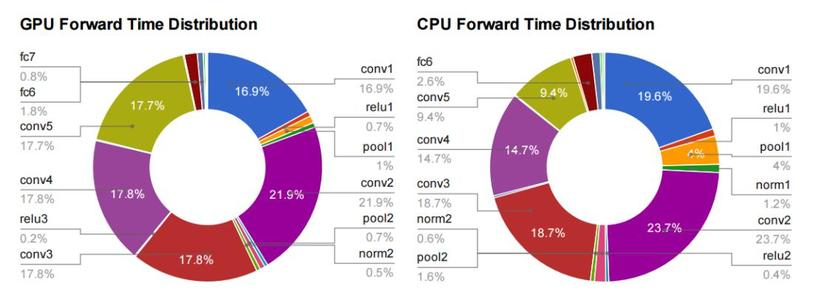
\includegraphics[width=0.8\textwidth]{GPU-CPU_compute_compare.jpg}
	\caption{GPU-CPU运算时间分布}
	\renewcommand\figurename{图}
\end{figure}
如图1所示,是AlexNet网络中不同的层在GPU和CPU中的运算时间消耗,可以明显看到,无论是在GPU还是CPU上最耗时的层是卷积层,因此,若要明显改善网络的运算性能,就要提高卷积层的计算效率。
\subsection{模型压缩策略}

\subsection{改变卷积方式策略}














		

\section{参考文献}

\renewcommand\refname{}

\bibliographystyle{unsrt}

\bibliography{ref}	
\end{document}